\newpage
\section{Auswertung}
\subsection{Bragg Bedingung}

\begin{figure}
    \centering
       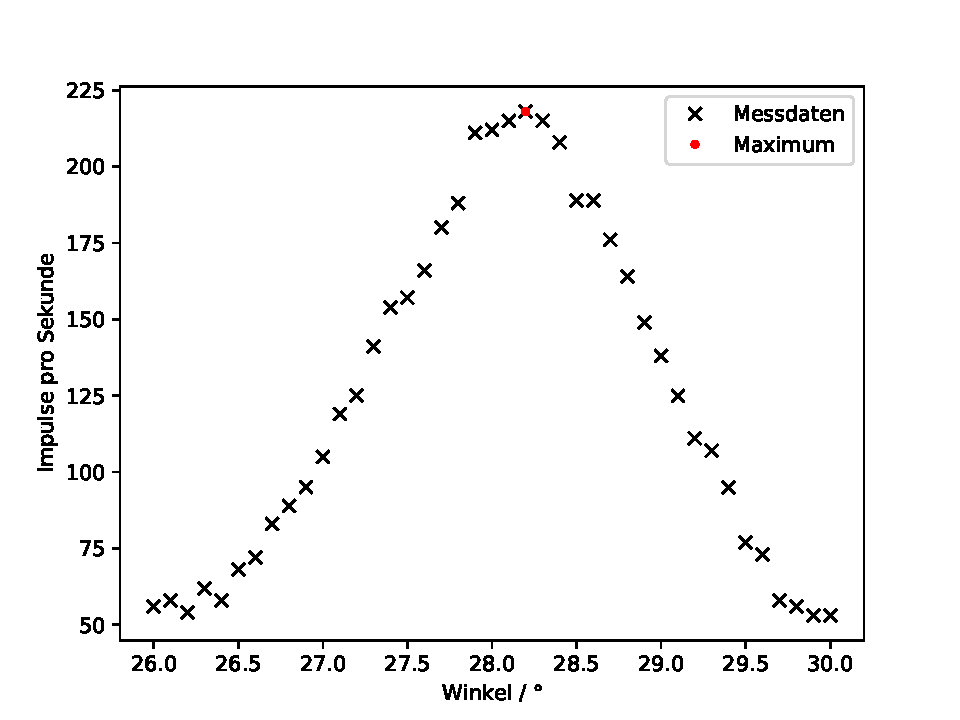
\includegraphics[height=9cm]{daten/Bragg.pdf}
       \caption{N gegen $\theta$ aufgetragen.}
       \label{fig:bragg}
\end{figure}

\noindent
Aus (\ref{fig:bragg}) wird ein Maximung bei einem Winkel von $\theta=28.2°$ ermittelt.
Daraus lässt sich die absolute und relative Abweichung vom Sollwinkel bestimmen.

\begin{align*}
\Delta\theta_{\text{abs}}&=0.2°\\
\Delta\theta_{\text{rel}}&=0.0071=0.7\%
\end{align*}

\subsection{Emissionsspektrum}
\noindent
Aus den Messdaten lässt sich das Emissionsspektrum einer Kupferröntgenröhre in (\ref{fig:emi}) graphisch darstellen.


\noindent
Zu erkennen sind die ermittelten Peaks, die die $\text{K}_\alpha$ und $\text{K}_\beta$ Linie darstellen, sowie der rot makierte Bremsberg.

\noindent
Die maximale Energie $\text{E}_\text{max}$ und die minimale Wellenlänge lassen sich aus der Beschleunigungsspannung U=35 $\si{\kilo\volt}$ bestimmen. 
Mit (xx) ergibt sich für den Grenzwinkel dann:

\begin{align*}
    \text{E}_\text{max} &= 35 \, \mathrm{keV}\\
    \lambda_\text{min} &= 354.241 \, \mathrm{nm}\\
    \theta_\text{Grenz} &= 5.045°
\end{align*}


\begin{figure}
    \centering
       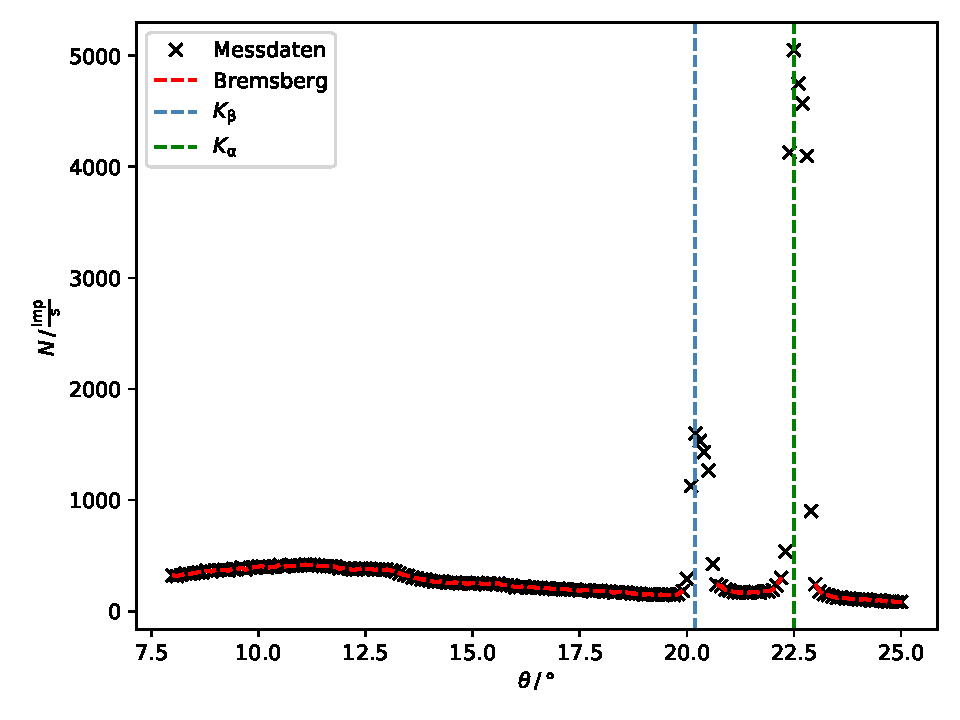
\includegraphics[height=9cm]{daten/emissionsspektrum.pdf}
       \caption{Emissionsspektrum einer Cu-Röntgenröhre.}
       \label{fig:emi}
\end{figure}

\noindent
Das Detailspektrum um die Peaks ist in (\ref{fig:emi2}) dargestellt, wobei der grüne Bereich die Full Width at Half Maximum makiert.

\begin{figure}
    \centering
       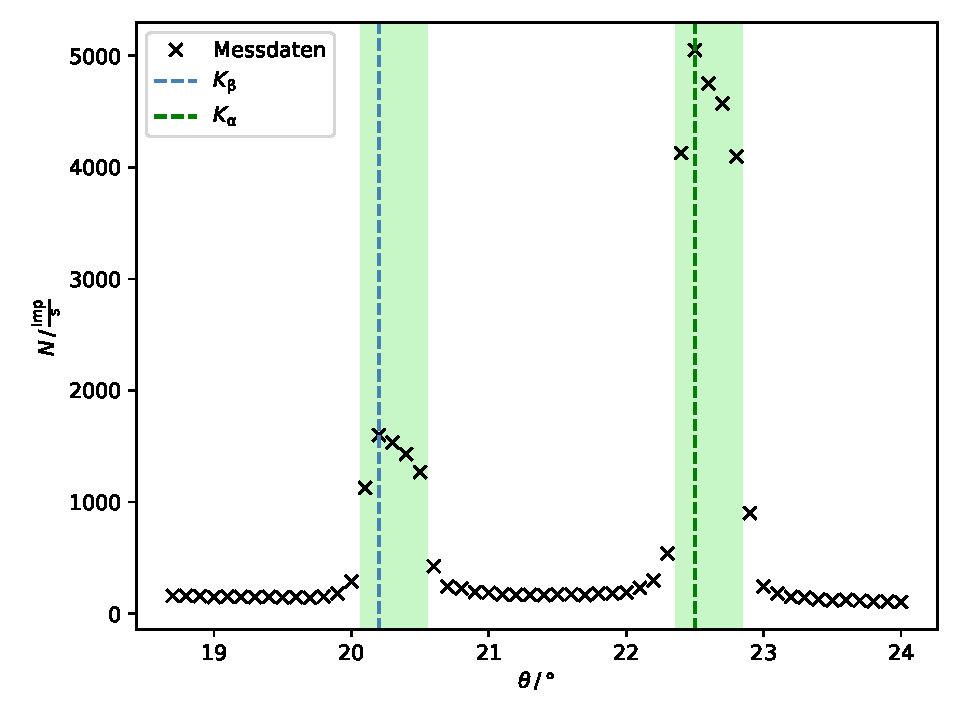
\includegraphics[height=9cm]{daten/emissionsspektrum2.pdf}
       \caption{Emissionsspektrum einer Cu-Röntgenröhre mit der FWHM.}
       \label{fig:emi2}
\end{figure}

\noindent
Hieraus lässt sich $\Delta\text{E}_{\text{FWHM}}$ bestimmen und daraus das Auflösungsvermögen A mit 

\begin{equation*}
\text{A}=\frac{\text{E}_{\text{max}}}{\Delta\text{E}_{\text{FWHM}}}
\end{equation*}

\noindent
für die $\text{K}_\alpha$ und $\text{K}_\beta$ Linie berechnen.
So ergibt sich:

\begin{align*}
\theta_\alpha&=20.2° & \theta_\beta&=22.5° \\
\text{E}_\alpha&=8.0434 \, \mathrm{keV}   &\text{E}_\beta&=8.9142 \, \mathrm{keV} \\
\Delta\text{E}_{\text{FWHM}\alpha}&=165.63 \, \mathrm{V}   &\Delta\text{E}_{\text{FWHM}\beta}&=205.58 \, \mathrm{V} \\
\text{A}_\alpha&=48.56  &\text{A}_\beta&=43.36 \\
\end{align*}

\noindent
Mithilfe der aus der Literatur entnommenen Absorptionsenergie $\text{E}_\text{K,abs} = 8980.476 \, \mathrm{eV}$ 
können die Abschirmkonstanten für Kupfer mit den Formeln 

\begin{equation*}
\sigma_1=Z-\sqrt{\frac{E_{Kabs}}{R_y}}
\end{equation*}

\begin{equation*}
\sigma_2=Z-\sqrt{ \frac{m^2}{n^2}(Z-\sigma_1)^2 - \frac{m^2}{R_\infty} E_{K\alpha}}
\end{equation*}

\begin{equation*}
    \sigma_3=Z-\sqrt{ \frac{l^2}{n^2}(Z-\sigma_1)^2 - \frac{l^2}{R_\infty} E_{K\beta}}
\end{equation*}
    


\noindent
bestimmt werden. Mit n=1, m=2 und l=3 ergeben sie sich zu:

\begin{align*}
    \sigma_1 &= 3.3031° \\
    \sigma_2 &= 12.3981°\\
    \sigma_3 &= 22.3776°
\end{align*}

\subsection{Das Absorptionsspektrum}

\noindent
Im Folgenden sind die K-Kanten von Zink, Gallium, Brom, Rubidium und Strontium aufgetragen.

\begin{figure}
    \centering
       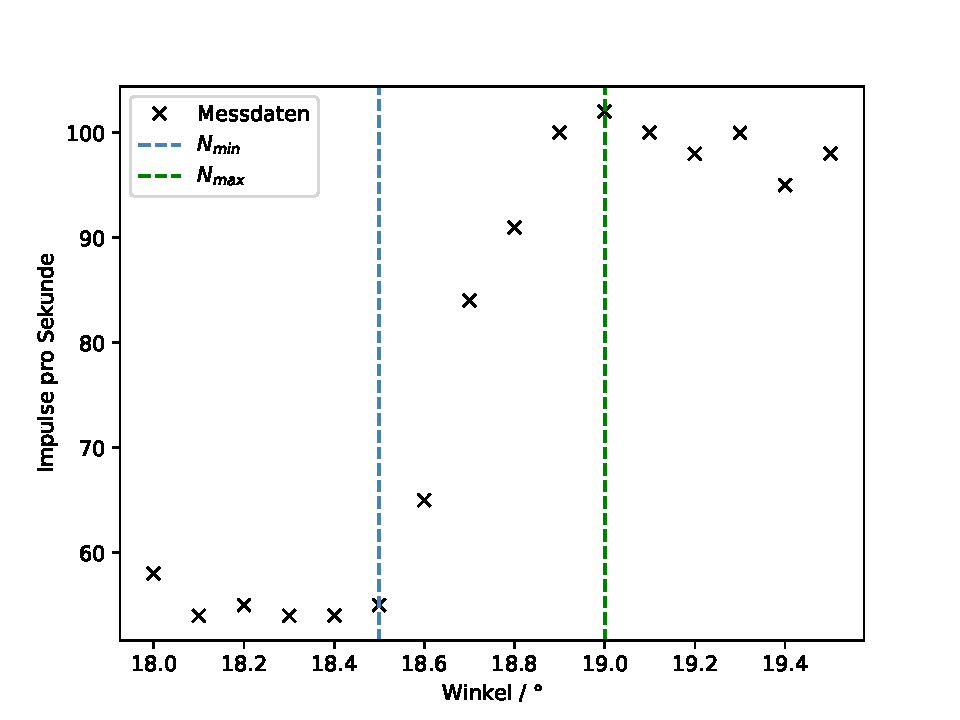
\includegraphics[height=9cm]{daten/zink.pdf}
       \caption{Absorptionsspektrum eines Zinkabsorbers.}
       \label{fig:zink}
\end{figure}

\begin{figure}
    \centering
       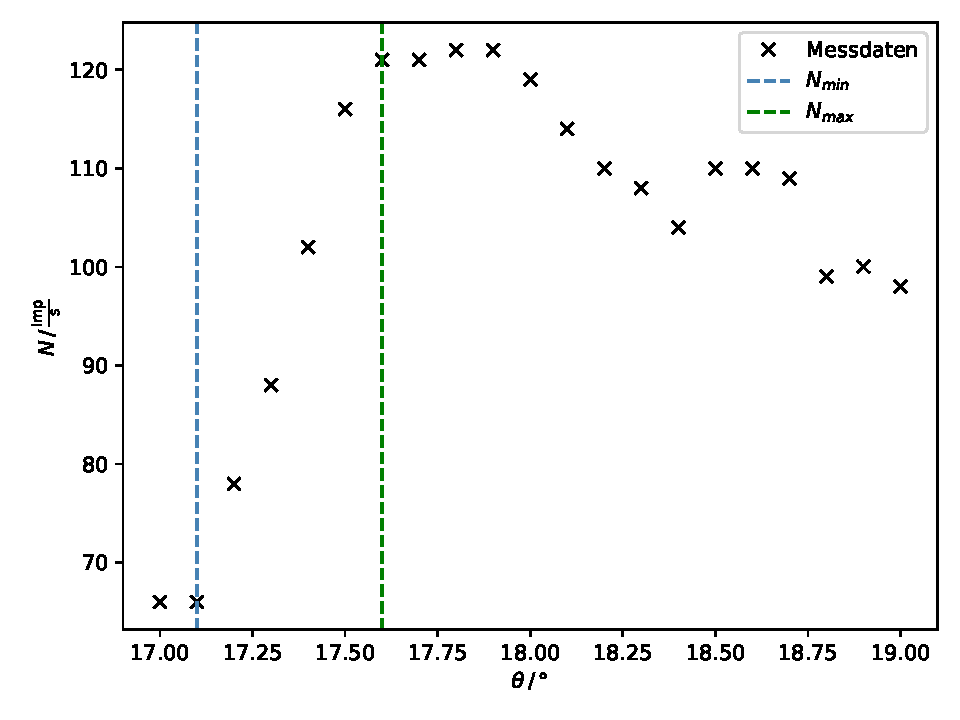
\includegraphics[height=9cm]{daten/gallium.pdf}
       \caption{Absorptionsspektrum eines Galliumabsorbers.}
       \label{fig:gallium}
\end{figure}

\begin{figure}
    \centering
       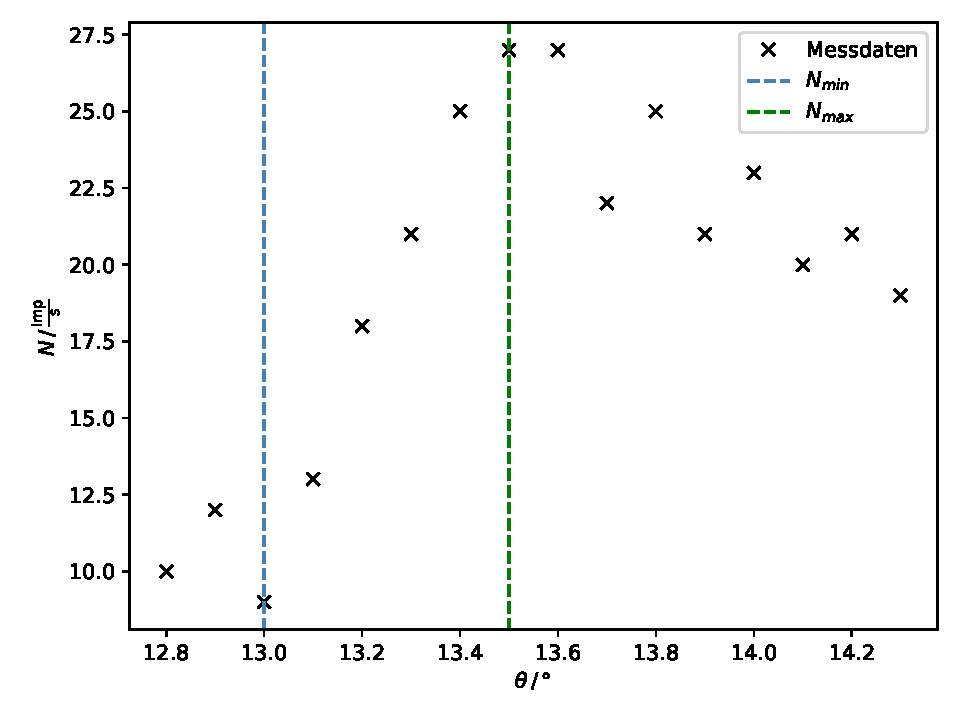
\includegraphics[height=9cm]{daten/brom.pdf}
       \caption{Absorptionsspektrum eines Bromabsorbers.}
       \label{fig:brom}
\end{figure}

\begin{figure}
    \centering
       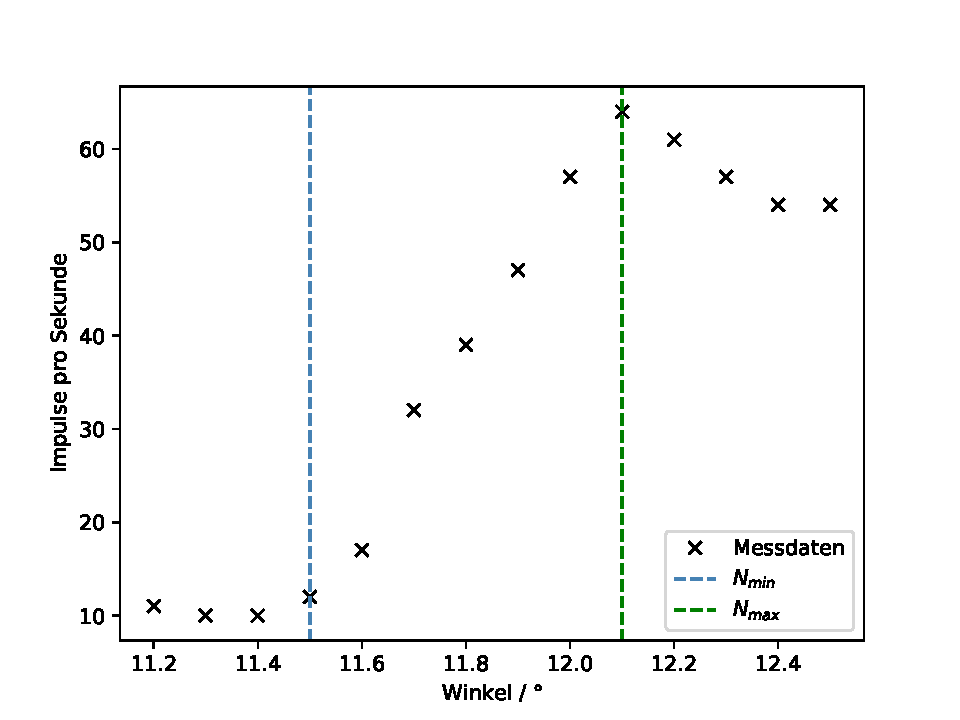
\includegraphics[height=9cm]{daten/rubidium.pdf}
       \caption{Absorptionsspektrum eines Rubidiumabsorbers.}
       \label{fig:rubidium}
\end{figure}

\begin{figure}
    \centering
       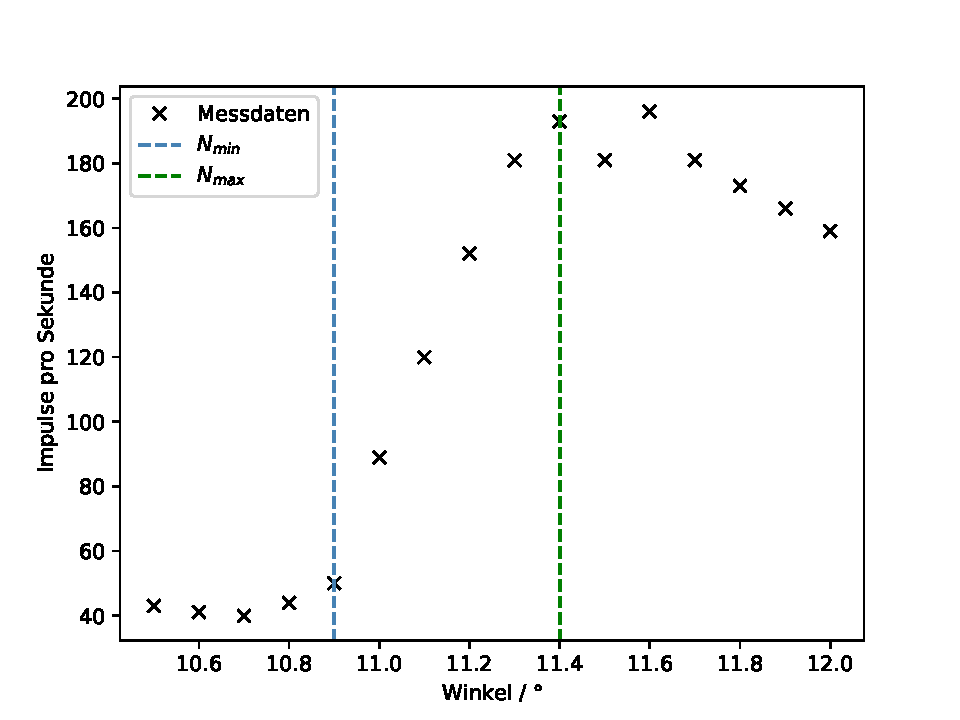
\includegraphics[height=9cm]{daten/strontium.pdf}
       \caption{Absorptionsspektrum eines Strontiumabsorbers.}
       \label{fig:strontium}
\end{figure}

\noindent
Aus den gemessenen K-Kanten lassen sich die Bragg-Winkel $\theta_\text{K}$ sowie die Energieübergänge bestimmen,
woraus sich die Abschirmzahlen $\sigma_\text{K}$ bestimmen lassen.

\begin{table}
    \centering
    \caption{Messwerte der Energieübergänge $\text{E}_\text{K}$, Bragg-Winkel $\theta_\text{K}$ und Abschirmzahlen $\sigma_\text{K}$}
    \label{tab:mess3}
    \sisetup{table-format=2.1}
    \begin{tabular}{c c c c c}
    \toprule
         & $\text{Z}$ & $\text{E}_\text{K} \,/\, \mathrm{keV}$ & $\theta_\text{K} \,/\, ° $ & $\sigma_\text{K} $\\
    \midrule 
      Zn & 30 & 9.6005  & 18.7 & 3.6345 \\
      Ga & 31 & 10.3508 & 17.3 & 3.6359 \\
      Br & 35 & 13.4795 & 13.2 & 3.8365 \\
      Rb & 37 & 15.0519 & 11.8 & 4.1091 \\
      Sr & 38 & 15.9881 & 11.1 & 4.1203 \\
    \bottomrule
    \end{tabular}
    \end{table}

Die Abweichungen zu den Literaturwerten für die Werte für Zink betragen somit:
\begin{align*}
    \Delta\text{E}_\text{abs}&=49.4578 \, \mathrm{keV} & \Delta\text{E}_\text{rel}&=5.13\%\\
    \Delta\theta_\text{abs}&=0.0996° & \Delta\sigma_\text{rel}&=0.54\%\\
    \Delta\sigma_\text{abs}&=0.0745 & \Delta\sigma_\text{rel}&=2.09\%
\end{align*}

\subsection{Bestimmung der Rydbergkonstante}    

\noindent
Aus der Beziehung $\text{E}_\text{K} \sim \text{Z}^2$ nach Moseley
kann die Rydbergenergie aus der Steigung des $ \sqrt{\text{E}_\text{K}}-\text{Z}$ Diagramms aus (\ref{fig:mose}) bestimmt werden.

\begin{figure}
    \centering
       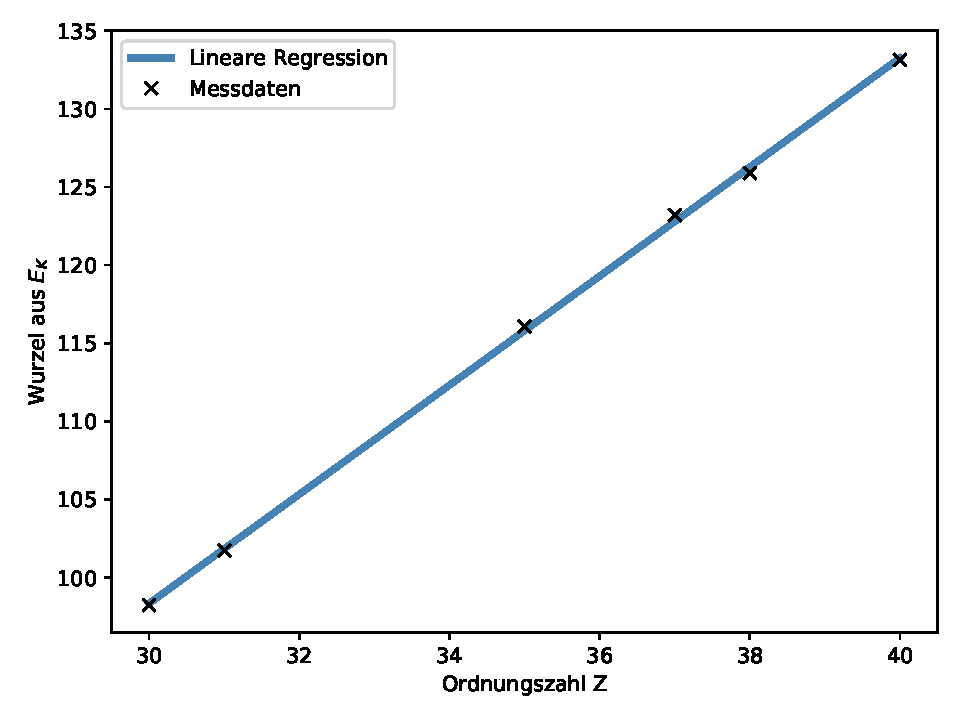
\includegraphics[height=9cm]{daten/mose.pdf}
       \caption{$\sqrt{\text{E}_\text{K}}-\text{Z}$ Diagramm.}
       \label{fig:mose}
\end{figure}

\noindent
Aus der Linearen Regression ergibt sich die Ausgleichsgerade

\begin{align*}
    g=3.5394\, x -8.0559.
\end{align*}

\noindent
Aus dem Quadrat der Steigung wird nun die Rydbergenergie zu 

\begin{align*}
    \text{R}_\infty =12.5271 \, \mathrm{eV}
\end{align*}

\noindent
bestimmt.
Daraus kann nun die Rydbergkonstante $\text{R}_\text{y}$ mit

\begin{equation*}
 \text{R}_\text{y}=\frac{\text{R}_\infty}{hc}
\end{equation*}

\noindent
zu 

\begin{align*}
\text{R}_\text{y} =10103826.71 \, \frac{1}{\text{m}}.
\end{align*}

\noindent
bestimmt werden.